\section{Generative Adevrsarial Networks}

Generative Adversarial Networks (GANs) is a novel framework for training generative models via an adversarial process
which was first introduced by \citet{GAN}.
In the paper , "Generative Adversarial Nets" , a generator network $G$ produces samples aimed at mimicking
the data distribution , while the discriminator $D$ estimates the probability of whether an input is real or generated \citep{GAN}.
In other words, GAN framework basically corresponds to a minimax two-player game where , 
a generator ($G$) creates samples that are intended to come from the same distribution as the training data, while the discriminator
$D$ examines the probability of the the samples provided by $G$ being real or fake \citep{goodfellow2017nips2016tutorialgenerative}.

\begin{figure}[htbp]
    \centering
    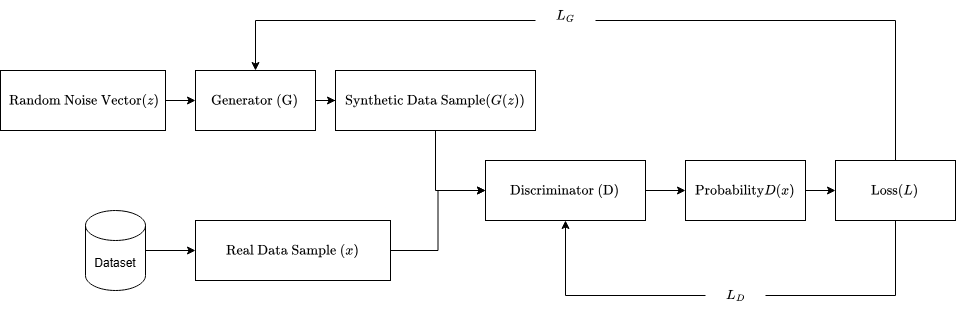
\includegraphics[width=1\linewidth]{figures/gan_framework.png}
    \caption{\textit{Generative Adversarial Networks (GANs) Architecture}}
    \label{fig:GanFramework}
\end{figure}

As shown in Figure~\ref{fig:GanFramework} the generator $G$ takes as input a random noise vector $z \sim p_z$
(usually drawn from a simple distribution such as uniform or Gaussian) and outputs a synthetic data sample $G(z)$.
The goal of $G$ is to map the "latent" noise distribution into the data sample $G(z)$ is as realistic as possible.
The discriminator $D$ takes a data sample $x$ as input and outputs a probability $D(x)$ estimating the likelihood that
$x$ is a real sample rather than one produced by $G$ \citep{salehi2020generativeadversarialnetworksgans,cohen2022generativeadversarialnetworks,Creswell_2018}.

The adversarial training process in GANs is governed by a minimax optimization. Formally, \citet{GAN} define the value function:
\[
V(D,G) = \mathbb{E}_{x \sim p_{\text{data}}(x)}[\log D(x)] + \mathbb{E}_{z \sim p_z(z)}[\log(1 - D(G(z)))]
\] and train $D$ and $G$ in a two-player game:
\[
\min_{G} \max_{D} V(D,G)
\]

$D$ and $G$ are alternatively updated via minibatch stochastic gradient descent during the GAN training process. 
$D$ is trained to maximize the probability of predicting whether an input from both training example and sample from G are real or fake,
while $G$ is trained simultaneously to minimize $\log(1-D(G(z)))$ \citep{GAN}. 
In reality, GAN training can be delicate: if $G$ becomes too strong or $D$ too weak , gradients can vanish, and if $D$ is too strong early on , $G$ may recieve no learning signal(saturating loss).
\citet{GAN}  suggest a non-saturating heuristic for $G$ (maximizing $\log D(G(z))$) instead of minimizing $\log(1-D(G(z)))$ to provide stronger gradients in practice. 

On its first introduction , GANs have brought about advantages compared to other generative models at the time (e.g. Variational Auto-encoders(VAE))
like sharper images, configurable sizes, richer search space, and a veratility as it can support different generator networks.
However it also has its disadvatages like : mode collapse, vanishing gradients , and instability \citep{cohen2022generativeadversarialnetworks}.

Since the original introduction of GANs, there have been many improvements in their architecture that have led to better image quality, 
more stable training, and expanded functionality. Early research highlighted how important convolutional structures are for making GANs 
work well. One of the most influential contributions came from \citet{richardson2021encodingstylestyleganencoder}, 
who proposed the Deep Convolutional GAN (DCGAN) along with a set of practical design tips for building effective convolutional GANs. 
Instead of relying on traditional pooling or unpooling layers, DCGAN used strided convolutions to reduce spatial resolution and 
transposed convolutions to increase it. This approach allowed both the generator and discriminator to learn spatial features 
more effectively, leading to more realistic outputs \citep{goodfellow2017nips2016tutorialgenerative}.
They also advocated batch normalization in almost all layers of both $G$ and $D$ (except the output and input layers, respectively),
which greatly stabilizes training and helps the models learn proper scales.
These guidelines enabled DCGANs to synthesize high-resolution images in “one shot” and to learn disentangled latent representations 
(e.g. enabling simple vector arithmetic in latent space to change semantic attributes of the output). 
DCGAN also popularized the use of Adam as the optimizer for GANs \citep{goodfellow2017nips2016tutorialgenerative}.

Over time, a proliferation of GAN variants has addressed different tasks and improved performance. 
Surveys note that variants include Conditional GANs (which incorporate label or conditional information), 
Wasserstein GANs (WGANs) (which replace the vanilla loss with an Earth-Mover distance for better gradients),
CycleGANs (for unpaired image-to-image translation), 
StyleGANs (which use style-based generator architectures for ultra-high-quality images), among many others \citep{Chakraborty_2024}.